\documentclass{acm_proc_article-sp}

\begin{document}

\title{Team building in Heterogeneous Groups of Humans and Robots}

\numberofauthors{3} %
\author{
% 1st. author
\alignauthor
Timothy Sweet\\
       \affaddr{University of Nevada, Reno}\\
       \affaddr{1664 North Virginia Street}\\
       \affaddr{Reno, Nevada 89557}\\
       \email{timothy.l.sweet@gmail.com}
% 2nd. author
\alignauthor
Jared Rhizor\\
       \affaddr{University of Nevada, Reno}\\
       \affaddr{1664 North Virginia Street}\\
       \affaddr{Reno, Nevada 89557}\\
       \email{me@jaredrhizor.com}
% 3rd. author
\alignauthor
David Feil-Seifer\\
       \affaddr{University of Nevada, Reno}\\
       \affaddr{1664 North Virginia Street}\\
       \affaddr{Reno, Nevada 89557}\\
       \email{dave@cse.unr.edu}
}

\maketitle
\begin{abstract}
Humans often engage in team building activities to improve cooperation between team members and promote positive group identity. As the field of robotics develops, humans will be required to work cooperatively with robots on many group tasks. In this paper, we explore the effect of team building activities on a group consisting of three agents: two human participants and one robot. The team building and primary tasks are chosen to be simple, generic, and representative of the kinds of collaborative activities heterogeneous robot and human teams might have to do.

We find that humans' perceptions of robots significantly improves after performing team building activities, and conclude that heterogeneous teams of humans and robots may be more successful at their tasks if they first perform team building activities.
\end{abstract}

%Tim doesn't know what these sections are suppose to be so he commented them out
% A category with the (minimum) three required fields
%\category{H.4}{Information Systems Applications}{Miscellaneous}
%A category including the fourth, optional field follows...
%\category{D.2.8}{Software Engineering}{Metrics}[complexity measures, performance measures]

%\terms{Collaboration}

\keywords{Team building, collaboration}

\section{Introduction}
\label{introduction}
Humans often engage in team building activities to improve cooperation between team members and promote positive group identity. For example, \cite{Rivas} reviewed current team building activities and determined that they provided ``a sense of unity and cohesiveness'' which improved the function of teams.

As the field of robotics develops, humans will be required to work cooperatively with robots on many group tasks. Some researchers have been exploring a variety of aspects of human-robot teamwork, ranging from how a robot should navigate \cite{Feil-Seifer} to dialogue structuring \cite{Fong}. 

When groups work together it is important to promote a collaborative atmosphere between all group members, including mixed groups of humans and robots. Team building is a tool regularly used to promote this collaborative atmosphere. Including robots in team building exercises extends human group interactions to human and robot group interactions. Our study investigates the introduction of team building into a group consisting of two humans and a robot, and how this introduction changes the perceptions of each member of the group (human and robot).

The rest of this paper is organized as follows. Section \ref{section:related-work} presents previous related work to robot and human team building. Section \ref{section:aim-of-the-experiment} presents our hypothesis. Section \ref{experimental-methodology} presents our experimental methodology. Section \ref{section:objective-evaluation} presents an objective evaluation and subjective evaluation of our experiment results. Section \ref{section:results} presents a complete view of the results of our study. Section \ref{section:discussion} presents a discussion of the significance of our results. Section \ref{section:limitations-and-further-work} presents the limitations of our study and possible further research based on our experiment. The paper is concluded in Section \ref{section:conclusions}.

\section{Related Work}
\label{section:related-work}
Previous research completed relating to this study is centered around three areas: one human and one robot interaction, human-only team building, and heterogeneous human-robot teams. 

Research involving one human and one robot interaction can focus on the usage and design of a specific robot or how activities or circumstances change the behaviors and perceptions of both humans and robots. In this work, we focus on the latter. Specifically, this paper focuses on deliberately non-anthropomorphic robots. This approach was inspired in part by \cite{Unhelkar}, which used an industrial robot as platform to evaluate how fluidity, comfortableness, and noticablility changed with several parameters in fetch-and-deliver tasks involving a robot and a human. The robot and human work collaboratively to complete a simple task. The robot has very limited communication with the human counterpart, which is a believable real-world constraint.
\cite{Fong} uses the concept of presenting a robot as a partner instead of a tool. Although we do not extend this concept to collaborative control like Fong, we actively choose to introduce the robot as a third participant in the study, i.e. a partner.

The field of education research contains most team building studies and reports. \cite{Rivas} shows that team building activities serve as a bridge between meeting people and completing an activity, helping to build ``trust and connectedness.'' The team building activities described by Rivas involve a structured setting in which the participants must describe some aspect of themselves to other participants. \cite{Dyer} also refers to team building exercises as a proven way to increase the performance of human groups.

The area heterogeneous human-robot teams often involves organization and planning for large teams. \cite{Ponda} is a prime example of work to orchestrate heterogeneous collaborative tasks. While creating group plans to achieve tasks, we believe that this is a separate problem compared to unifying a heterogeneous team before a task. With the Wizard of Oz approach, we accomplish human-like planning for the robot. 

Additionally, \cite{Godspeed} investigates measures used to evaluate robots. Animacy, likeability, perceived intelligence, and other measures are suggested as areas to evaluate within HRI. We found many of these metrics are used in the Godspeed Questionairre, which we use to evaluate participants' experiences with the robot and with the other participant.

\section{Aim of the experiment}
\label{section:aim-of-the-experiment}
We investigate the interactions between a heterogeneous team of two humans and robot performing one or two simple tasks. The tasks are a team building game, specifically the popular ``Two Truths and One Lie'', and the primary object finding task. Through the experiment we seek to evaluate the following hypotheses:
\begin{itemize}
 \item \textbf{H1} A human's perception of a robot will improve after participating in team building with the robot
 \item \textbf{H2} The human unsuccessful at the primary task will perceive the robot better than a human successful at the primary task will perceive the unsuccessful human.
\end{itemize}

\begin{figure}[here]
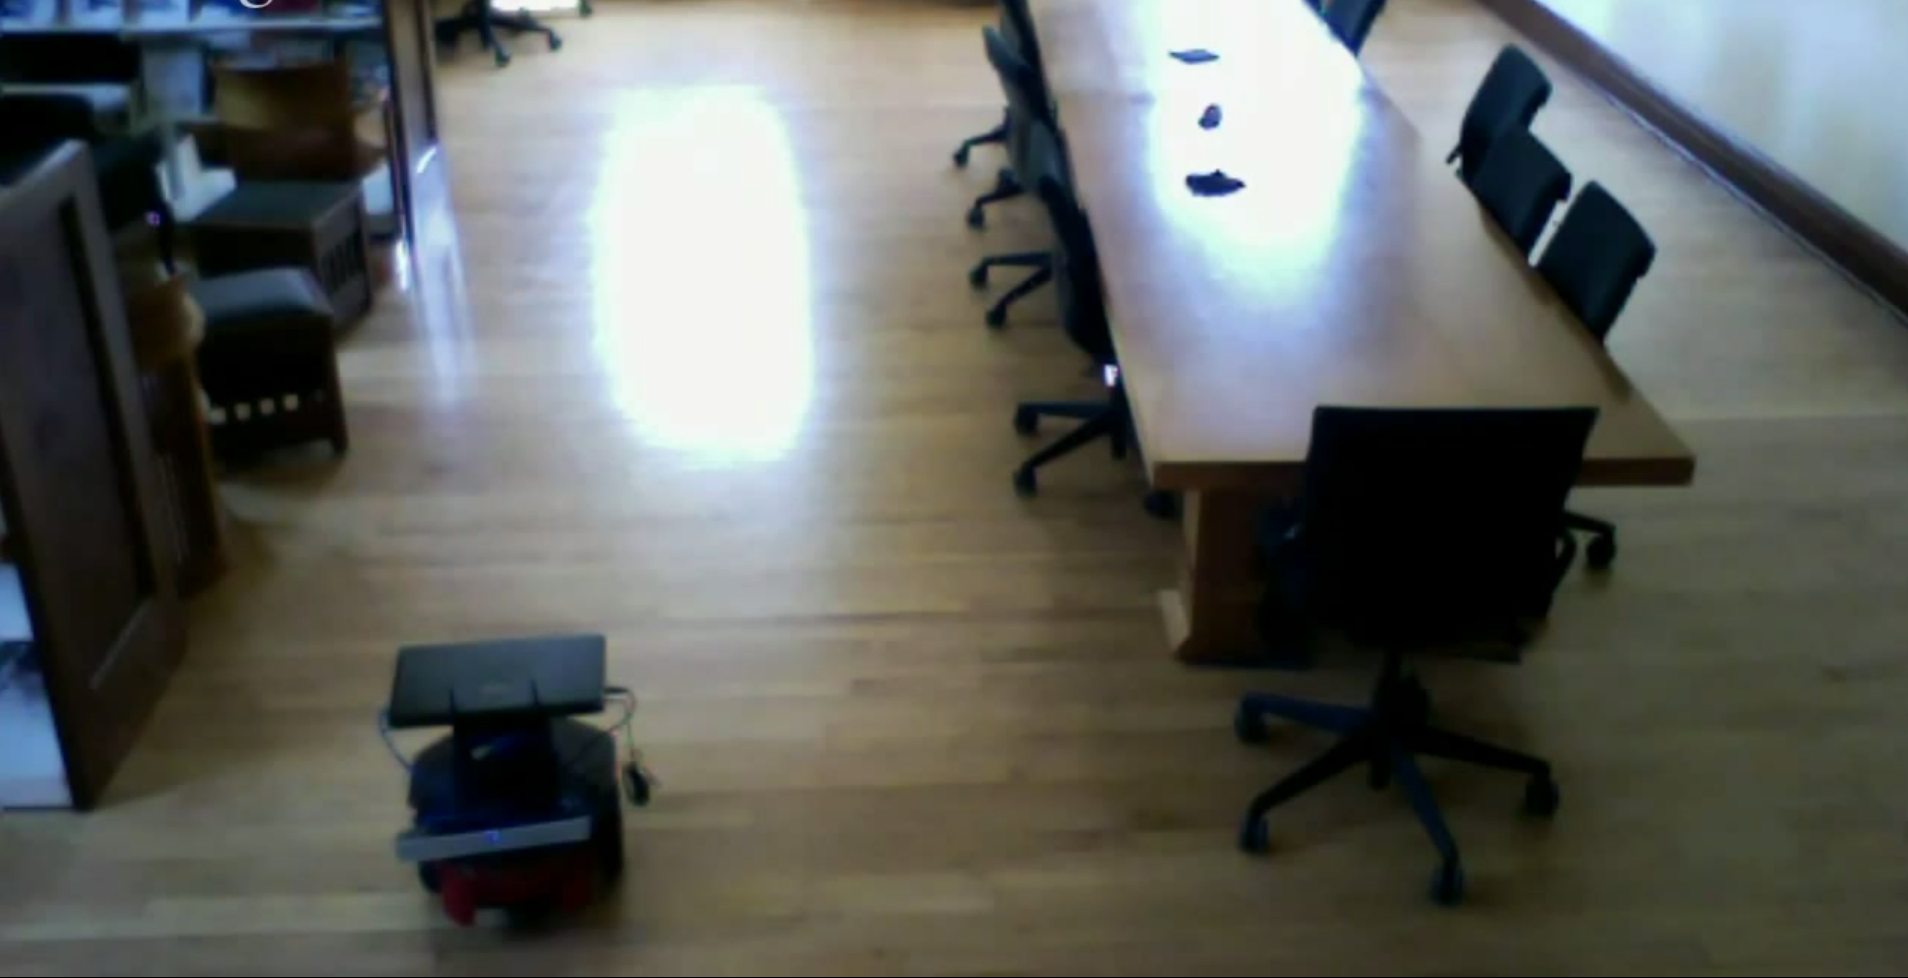
\includegraphics[width=0.45\textwidth]{camera.png}
\caption{The location of the study.}
\label{fig:studylocation}
\end{figure}

\section{Experimental Methodology}
\label{experimental-methodology}
The experiment is designed to represent a simple task in which teamwork between humans and a robot would increase the probability of the task's success compared to the humans working alone. This is meant to be representative of many real-world activities requiring human and robot teamwork. In this task, the team consisting of two humans and one robot are instructed to locate a particular object in a large room (Figure~\ref{fig:studylocation}). The participants are told the robot is capable of detecting when it can ``see'' the object with its camera, and thus the robot will be able to help find the object. Participants are subject to a time limit, increasing the difficulty of finding the object.

\begin{figure}[here]
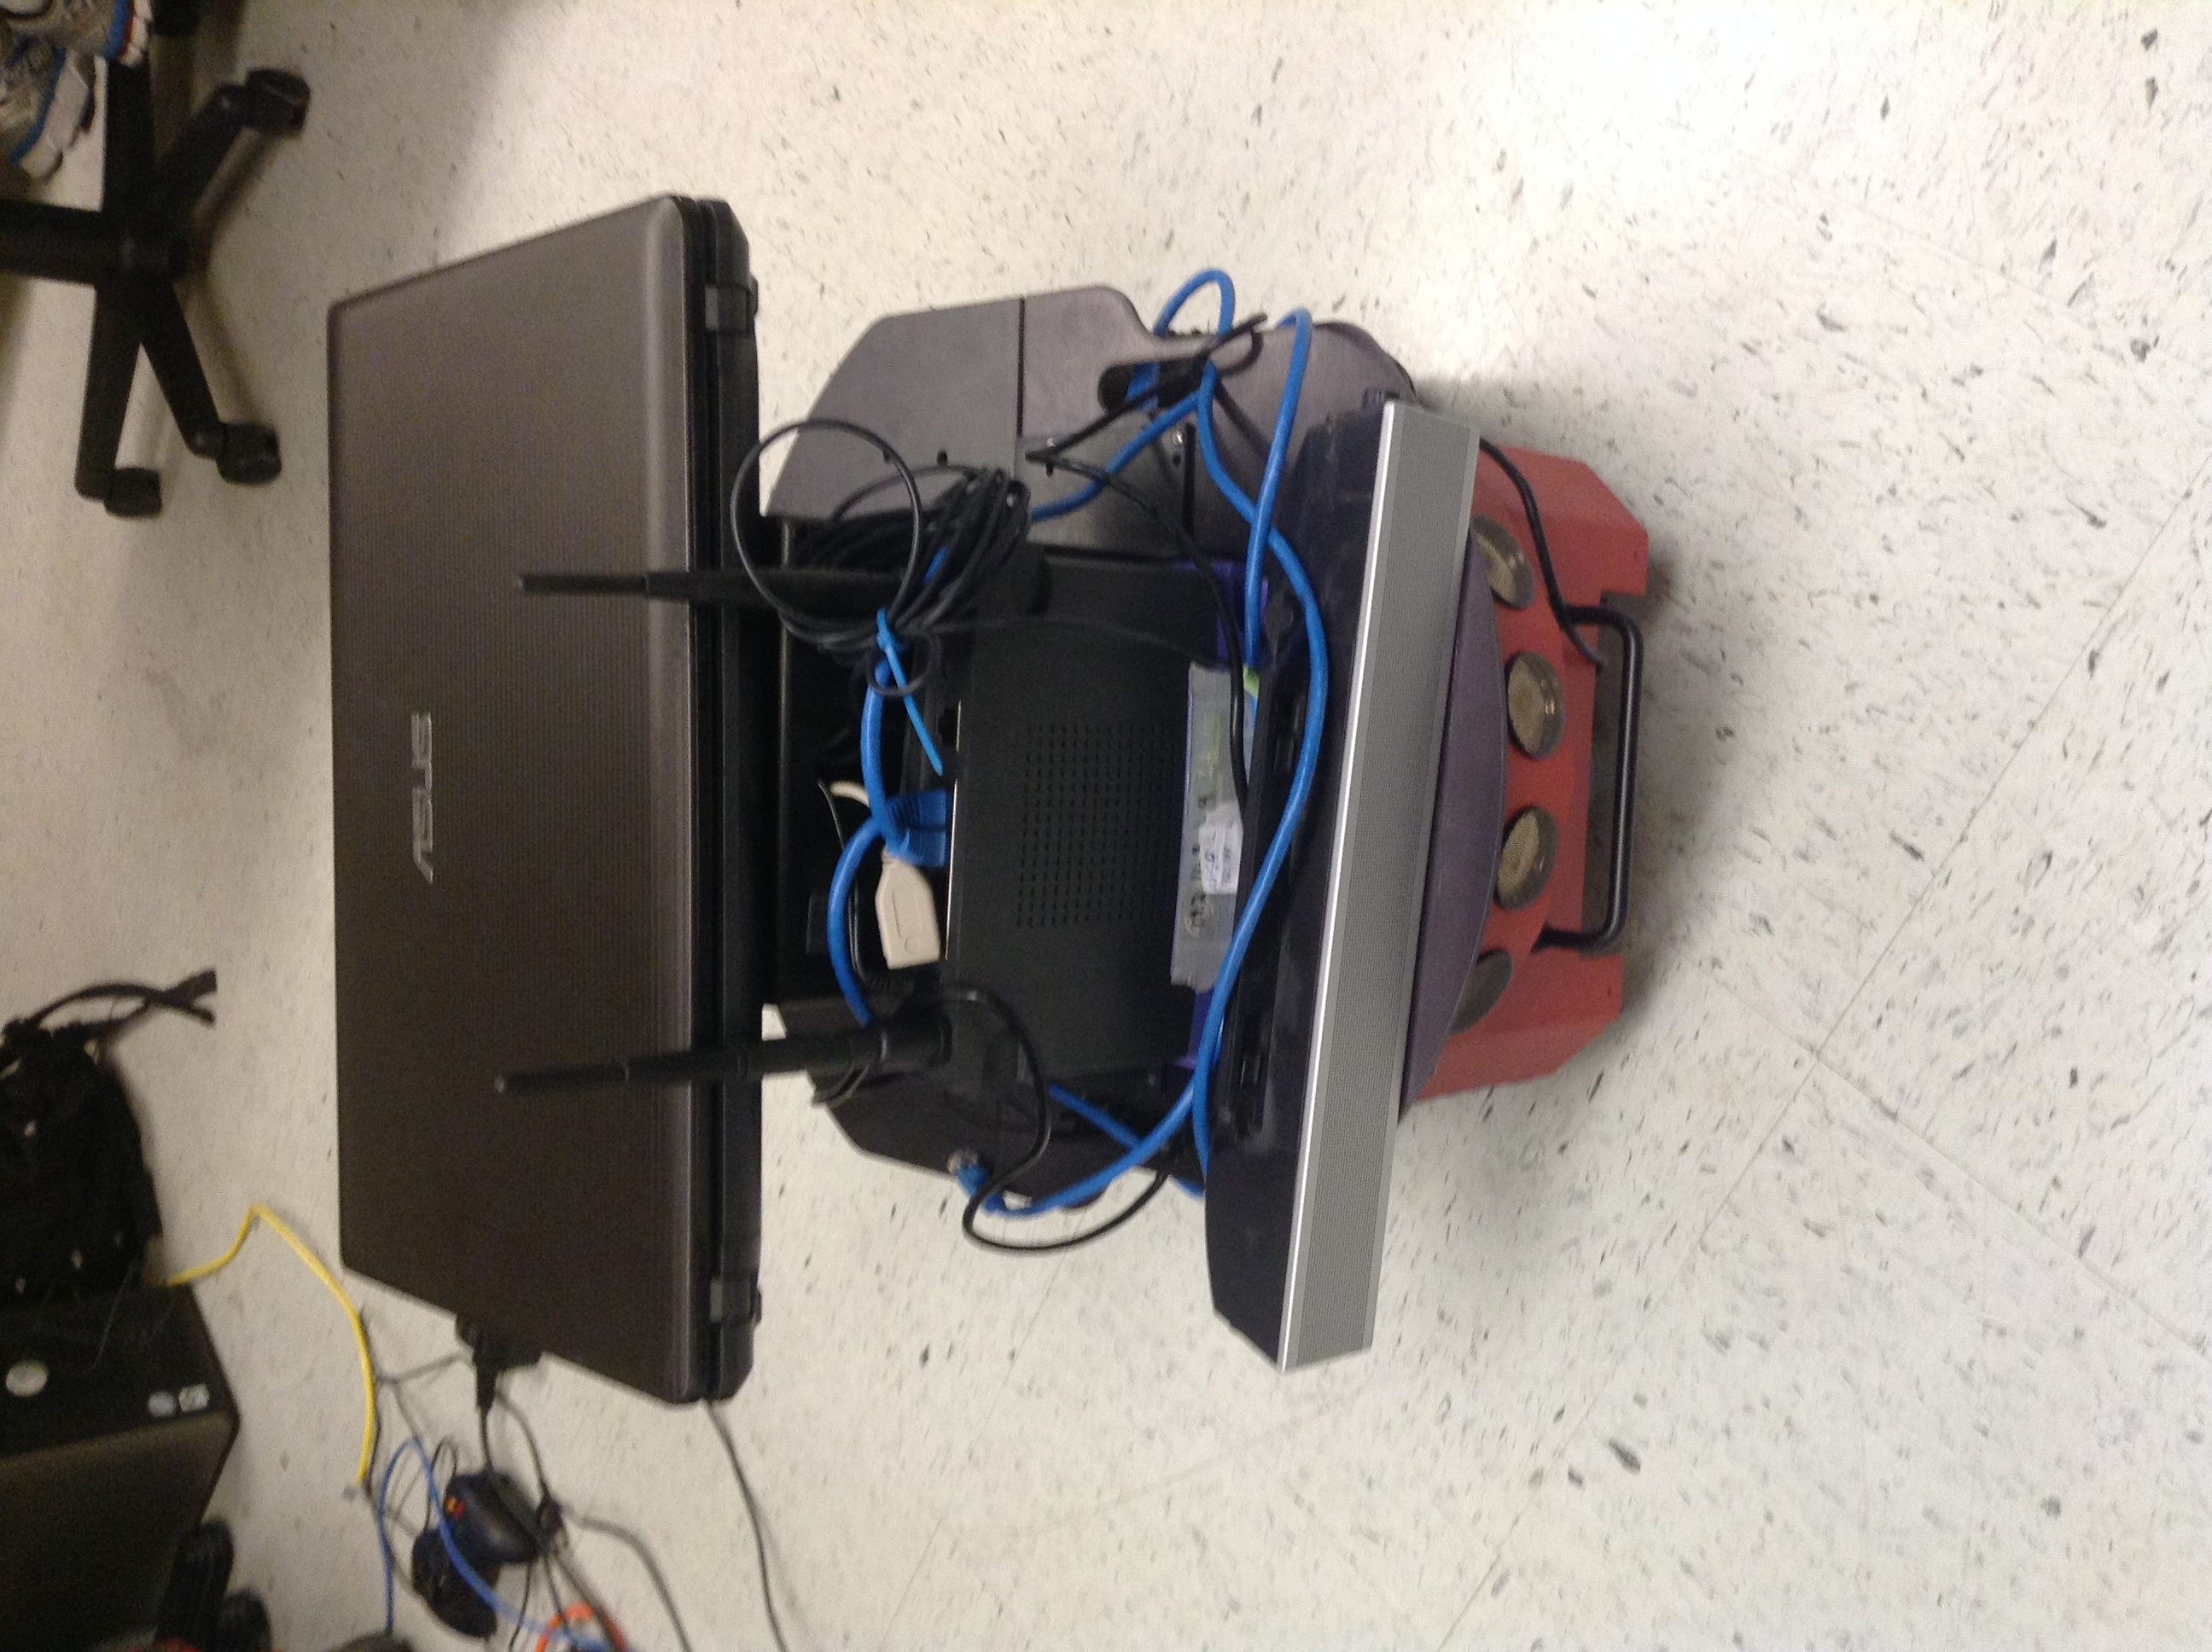
\includegraphics[width=0.45\textwidth]{robot.png}
\caption{The robot with the attached laptop, SICK laser, router, and speaker.}
\label{fig:robot}
\end{figure}

\subsection{Materials and Setup}
The Adept MobileRobotics Pioneer 3DX shown in Figure~\ref{fig:robot} is used as the robotic base for the experiment. It is equipped with a SICK LMS 100 Laser Rangefinding for navigation, an Xtion Pro Live for detecting the object it is looking for, and additional computational components. A laptop running the Robot Operating System and laser processing is mounted on the Pioneer. The robot's onboard Raspberry Pi is controlled from a separate computer in a different room by a human (participants are unaware of this Wizard of Oz usage: they are led to believe the robot is navigating autonomously).

The room is a large library study room, set up to be sufficiently cluttered that finding an object takes some time. The object used is a blue whiteboard marker, chosen because it is easily concealable but also easily recognizable to both the humans and the robot's camera due to its bright color. The object is hidden such that the robot would be able to see it.

A Macbook Pro webcam was used to record audio and video for the duration of the study. 
\subsection{Team building activity}
\label{section:team-building-activity}
Some participants partake in a team building activity with the robot. This activity is the popular ``Two Truths and One Lie'' icebreaker. Each participant tells the group two truths and one lie about themselves, then their human teammate and the robot guess which statement was a lie, in that order. Unknown to participants, the remote human operator actually just plays a sound clip from the robot's onboard speaker which states ``I believe your second/third statement was a lie'' for the first and second human teammate, respectively, regardless of their statements. Finally, the remote operator plays a sound clip on the robot which states its two truths and a lie:
\begin{itemize}
 \item I was manufactured in 2003 (truth)
 \item I have traveled outdoors (truth)
 \item I can travel up to two meters per second (lie)
\end{itemize}
Participants then guess which statement was a lie, and the remote operator plays a sound clip stating ``I can only travel one meter per second''. The team building activity is now concluded.

The facilitator within the room gestures at each participant when it is their turn to speak (both humans and the robot). The remote operator can see the facilitator gesture on the video feed, which is used as the cue for each sound clip to play.

Note that we avoid anthropomorphizing the robot because this study does not focus on human-like robots. The voice used in every audio clip is a very ``machine-like'' voice.
\subsection{Primary activity}
\label{section:primary-activity}
All participants partake in the primary activity. In this activity, participants are told that there is a blue white board marker hidden in the room somewhere. They are given sixty seconds to find it, with the help of their human partner and the robot. Participants are told the robot will announce ``I found it'' if it finds the marker, however the robot is actually being driven by the remote operator and will not announce if it ``sees'' the marker. In some cases the marker is actually hidden in the room, in other cases the marker is not in the room (thus the participants will run out of time before finding the marker). 

\begin{figure}[here]
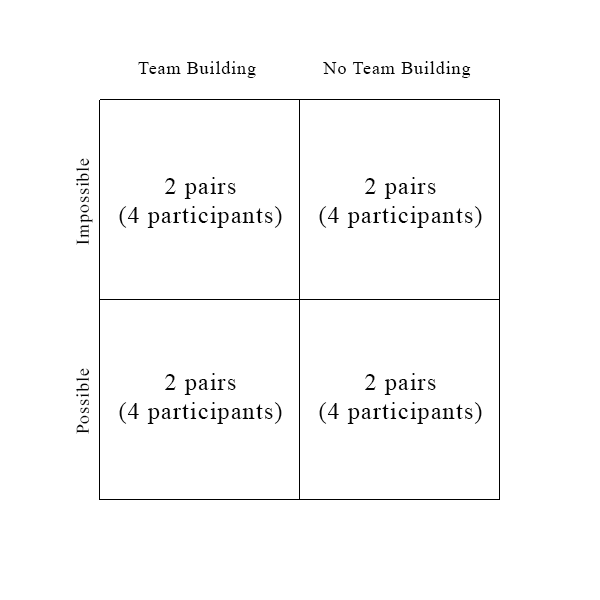
\includegraphics[width=0.45\textwidth]{participants.png}
\caption{The distribution of participants in each of the four cells.}
\label{fig:participantdistro}
\end{figure}

\subsection{Procedure}
Sixteen participants are recruited from our university library at random and asked if they would participate in a study in human-robot interaction. Two participants at a time are brought into the study room and consented, then introduced to each other and the robot. The participants are only asked to state their name, and the facilitator introduces the robot as ``a Pioneer 3DX''. Participants are asked if they have met each other and are dismissed or re-paired if so until the partners do not know each other. In other words, we control for familiarity between participants. We then tell the participants the robot is capable of finding the blue marker by placing it in front of the robot while the robot operator plays a sound clip stating ``I found it'' from the robot's onboard speaker. Thus the camera is not actually used for detection, the remote operator uses the Wizard of Oz method to create this effect. This was chosen to reduce the probability of technical difficulties in demonstrating the robot's competency.

Participants are then separated and asked to fill out the Godspeed Questionnaire \cite{Godspeed} with respect to their human teammate and again for their robotic teammate. After completion, they are brought back together in the main study room.
Half of the participants partake in the team building activity described in Section \ref{section:team-building-activity}. Then, all participants partake in the primary activity described in Section \ref{section:primary-activity}, and in half of those cases the task is possible and in the other half it is impossible. Thus, there are four studied cells:
\begin{itemize}
 \item Possible task with team building activity
 \item Possible task without team building activity
 \item Impossible task with team building activity
 \item Impossible task without team building activity
\end{itemize}

Figure~\ref{fig:participantdistro} contains a graphic describing the distribution of participants among the cells. 

After finishing the primary activity, participants are separated again and asked to fill out the same Godspeed questionnaire for their human teammate and again for their robotic teammate. After finishing the questionnaire participants are debriefed and dismissed. The facilitator uses a script throughout the experiment, but is allowed to respond to participant questions. 

\section{Evaluation}
\label{section:objective-evaluation}
Each participant filled out the Godspeed Questionnaire for each of their teammates twice: once at the beginning of the study and once at the end of the study. This is designed to evaluate the change in perception of each teammate after being exposed to the test conditions.
\subsection{Data Analysis Method:}
The participant responses were post-ordered such that higher numbered scores indicate more human-like and/or positive attributes, such as ``alive'' as opposed to ``dead'' and ``friendly'' as opposed to ``unfriendly''. With this ordering, we analyze each participant's responses for a particular teammate during the pre and post survey, and classify each response as ``more positive'', ``unchanged'', or ``more negative''. We also analyze the net change in a participant's perception of a particular teammate by similarly comparing the average of all scores in each survey.

\subsection{Subjective Data Collection:}
The facilitators wrote descriptions about any unexpected occurences within the study. Video of some sessions were reviewed to provide additional insight into certain participant interactions. These observations include any non-scripted facilitator-human or facilitator-robot interactions. 

\section{Results}
\label{section:results}

\subsection{Human Partner - Without Team building}
We first inspect the participants' responses to the survey regarding their human teammate. For cells with no team building we found the following average results:
\begin{itemize}
 \item Three participant's perception of their human partner did not change
 \item Three participant's perception of their human partner became more positive
 \item Two participant's perception of their human partner became more negative
\end{itemize}
These data indicate that the primary task had no noticeable or consistent impact on participants' perception of each other. Interestingly, there was no significant change in participants' perceptions of each other based on whether they found the marker or not.  Table \ref{table:HNT} indicates each participant's change in perception of their human teammate for this cell.

\begin{table}
\centering
\caption{Human Partner - Without Team building}
\begin{tabular}{|r|r|r|r|r|r|r|r|r|} \hline
&1.1&1.2&2.1&2.2&3.1&3.2&4.1&4.2\\ \hline
$\Delta$&0.00&-0.13&0.13&0.00&0.22&-0.04&0.00&0.39 \\ \hline
\end{tabular}
\label{table:HNT}
\end{table}

\subsection{Human Partner - With Team building}
For cells with team building we found the following average results:
\begin{itemize}
 \item One participant's perception of their human partner did not change
 \item Seven participant's perception of their human partner became more positive
 \item Zero participant's perception of their human partner became more negative
\end{itemize}
These data indicates that the human's perception of their human partner almost unanimously became more positive after team building, which supports the findings from prior work. Although the task given to participants 8.1 and 8.2 was possible (the marker was in the room) they did not find it in the prescribed amount of time, thus there is insufficient data to determine if the humans' perception of each other changed after the team building and primary task. Table \ref{table:HT} indicates each participant's change in perception of their human teammate in this cell.

\begin{table}
\centering
\caption{Human Partner - With Team building}
\begin{tabular}{|r|r|r|r|r|r|r|r|r|} \hline
&5.1&5.2&6.1&6.2&7.1&7.2&8.1&8.2 \\ \hline
$\Delta$&0.13&0.00&0.48&0.74&0.22&0.26&0.13&0.39 \\ \hline
\end{tabular}
\label{table:HT}
\end{table}

\subsection{Robotic Partner - Without Team building}
We next inspect the participants' regarding their  robotic teammate. For cells with no team building we found the following average results:
\begin{itemize}
 \item Zero participant's perception of their robotic partner did not change
 \item Four participant's perception of their robotic partner became more positive
 \item Four participant's perception of their robotic partner became more negative
\end{itemize}
These data indicate that that the primary task had no noticeable or consistent impact on the participants' perception of the robot. Table \ref{table:RNT} indicates each participant's change in perception of their robotic teammate in this cell.

\begin{table}
\centering
\caption{Robot Partner - Without Team building}
\begin{tabular}{|r|r|r|r|r|r|r|r|r|} \hline
&1.1&1.2&2.1&2.2&3.1&3.2&4.1&4.2\\ \hline
$\Delta$&0.57&-0.48&0.48&0.17&-0.22&-0.17&-0.04&0.04 \\ \hline
\end{tabular}
\label{table:RNT}
\end{table}

\subsection{Robotic Partner - With Team building}
For cells with team building we found the following average results:
\begin{itemize}
 \item Zero participant's perception of their human partner did not change
 \item Eight participant's perception of their human partner became more positive
 \item Zero participant's perception of their human partner became more negative
\end{itemize}
These data strongly indicate that the human's perception of their robotic partner unanimously became more positive after team building. Table \ref{table:RT} indicates each participant's change in perception of their robotic teammate in this cell.

\begin{table}
\centering
\caption{Robot Partner - With Team building}
\begin{tabular}{|r|r|r|r|r|r|r|r|r|} \hline
&5.1&5.2&6.1&6.2&7.1&7.2&8.1&8.2 \\ \hline
$\Delta$&1.04&0.17&0.70&0.52&1.26&0.04&0.35&0.26 \\ \hline
\end{tabular}
\label{table:RT}
\end{table}


\section{Discussion}
\label{section:discussion}
The results of our experiment support our hypothesis \textbf{H1} that the humans' perception of the robot will improve after performing team building, as exhibited by the unanimous increase (more-positive trend) in robot perception after team building. The humans' perception of the robot increased an average of 0.54 points on a 5-point Likert Scale with team building, compared to just 0.04 points without team building.
The results fail to support our hypothesis \textbf{H2} that the human unsuccessful at the primary task will perceive the robot better than a human successful at the primary task will perceive the unsuccessful human. This is partially due to a lack of data: one of the cases which should have yielded data related to this hypothesis failed when the participants did not find the object even though it was in the room(case 8). Section \ref{section:limitations-and-further-work} provides suggestions for further study on this hypothesis.

Some of the data contained interesting results outside of the two hypotheses. Participants who found the marker had a greater increase in perception of the robot than participants that did not find the marker. One possible explanation of this difference is that participants that found the marker felt more positive than the other participants after the task. If that explanation is true, then it is possible that intragroup competitiveness exists. While the task was intended to be and verbally staged as purely collaborative, finding the marker unduly affected the individual that found the marker and not the other participant.

\subsection{Observed Human Behavior}
\label{subsection:observed-human-human-behavior}
Some participants actively engaged with the other participant before being prompted to by the facilitator. During the script, when the participants are introduced by name, the participants shook hands with each other or initiated shaking hands with the facilitator. It is important to note that the participants were not instructed to limit their interactions with each other or the robot in any way. This lack of constraint was intended to make the situation more realistic; in general robot-human teams, the robot's communication abilities will be limited in some way, while humans can discuss anything, relevant to the task or not. 

During the one minute task itself, most participants verbally determined a plan to search the room by partitioning it into two regions. 

\subsection{Robot Capabilities}
\label{subsection:robot-capabilities}
The participants were not informed about the capabilities in the robot in any cell. This led to interesting interactions. Two participants talked to the robot during the task, trying to direct the robot in some way. One participant said ``Come here!'', trying to tell the robot to search an area where a low-set camera would be more suitable than a human crouching. 

The other participants simply observed the robot's actions and did not try to influence them. Some participants asked the facilitator about what the robot's camera could see.

Participants may have an inflated opinion of the robot's abilities due to the robot's high rate of success in the Two Truths and One Lie game. Almost all participants placed their lie in the second or third statement. Since the robot always guessed that the second statement was a lie for the first player in the game and that the third statement was a lie for the second player in the game, the robot guessed successfully as often as the other human participant. 

The only cases where the robot did not seem to be fully competent during the team building exercise was when a participant would use an observable truth (hair color, weather, etc.) in their statements. 

\subsection{Technical Difficulties}
\label{subsection:technical-difficulties}
In two runs of the study, a mistake was made by either the facilitator or the remote operator. Once, the robot did not ``locate'' the blue marker when it was placed in front of its PrimeSense sensor. This failure was due to the batteries dying on the robot laptop. The facilitator was clear to emphasize that he was to blame for the robot losing its charge and replaced the laptop with another, fully charged laptop. 

A second failure occurred the remote operator missed the cue to activate the text-to-speech. This was again blamed on the humans running the study for not ``starting the robot.'' In this way, any errors were clearly attributed to the individuals running the study, and not the robot itself in order to prevent the participants' perceptions of the robot from changing in a noticeability way. 

\section{Limitations and Further Work}
\label{section:limitations-and-further-work}
In order to confirm \textbf{H2} a significant number of participants need to be tested in that cell. Thus, it would be more effective for a future study to focus entirely on this cell to get a broader look at the range of opinions of participants.

Although the data solidly supported \textbf{H2}, an increase in the number and kind of participants would provide more insight into the effects of team building. All of the participants in the study were students at the University of Nevada, Reno. Groups of humans and robots working together will most likely be found in industrial applications in the near future. Focusing on this demographic may produce more applicable results. 

Another useful extension of this research would be to study the duration of team building effects on heterogenous groups of robots and humans. While we show that for very short interactions with a robot, human perception of the robot increases after team building, it is unclear whether or not these increased perceptions would be maintained throughout longer use of the robot or longer tasks. Additionally, it would be possible to study whether or not the human perception of the robot equalizes with and without team building over time. If perception does equalize, studying robot-human team building over time could reveal when team building is appropriate and worthwhile. 

In this study, the participant's state is unknown. A third part of each study could be created to have the participants rate themselves. The difference between these self-ratings and their partners' ratings (especially their robotic partners' ratings) could provide some insights into how the human participant relates to the robot, instead of how the human participant perceives the other participant relating to the robot. 

``Two Truths and One Lie'' seemed to be an effective team building activity with only a few exceptions. One participant struggled for about 30 seconds to come up with three statements. Even with the struggling, the participant did not have any significant difference in his or her responses. The activity went smoothly for the rest of the participants. However, if team building is going to be used regularly for heterogeneous teams, it is important to investigate other activities and how they can be applied to robots. In our literature review, we were unable to find scientific comparisons of different team building activities for human-only groups. Comparing multiple team building activities could reveal differences in effectiveness in different activities with respect to heterogeneous groups.

More statistical analysis could also be performed to analyze the data collected. Using analysis of variance could show how our data is partitioned mathematically, which should support our hypotheses and the conclusions reached in this paper.

\section{Conclusions}
\label{section:conclusions}
Human robot interactions will undoubtedly increase as the field of robotics advances. The use of heterogeneous groups of humans and robots will most likely increase over time as well. Since team building is viewed as an acceptable social activity to create cohesive groups of humans, team building with heterogeneous groups of robots and humans is a natural step forward. We show that humans tend to perceive robots better after team building activities than before. This trend is much stronger than the slight increase in perception of human partners after team building. Anecdotal observations and analysis of the data raise several important questions that should be addressed in the future. 


%ACKNOWLEDGMENTS are optional
\section{Acknowledgments}
\label{section:}
The authors would like to thank the DeLaMare Library for hosting our study, the University of Nevada, Reno Robotics Research Lab for allowing us to use the robotic equipment, as well as the student participants who volunteered their time during finals week.

%
% The following two commands are all you need in the
% initial runs of your .tex file to
% produce the bibliography for the citations in your paper.
\bibliographystyle{abbrv}

\begin{thebibliography}{}
\bibitem{Rivas} O. Rivas and I. S. Jones, ``Leadership: building a team using structured activities,'' Research in Higher Education Journal, vol. 17, 2012.
\bibitem{Feil-Seifer} D. J. Feil-Seifer and M. J. Matari\'{c}, ``People-Aware Navigation For Goal-Oriented Behavior Involving a Human Partner,'' in Proceedings of the International Conference on Development and Learning, Frankfurt am Main, Germany, 2011, pp. 1-6.
\bibitem{Fong} T. Fong, C. Thorpe, and C. Baur, ``Collaboration, Dialogue, and Human-Robot Interaction,'' in 10th International Symposium of Robotics Research, Lorne, Victoria, Australia, 2001, p. 255-266.
\bibitem{Godspeed} C. Bartneck, D. Kuli\'{c}, E. Croft, and S. Zoghbi, ``Measurement instruments for the anthropomorphism, animacy, likeability, perceived intelligence, and perceived safety of robots,'' International Journal of Social Robotics vol. 1, no. 1, 2009, pp. 71-81.
\bibitem{Unhelkar} V. V. Unhelkar, H. C. Siu, and J. A. Shah, ``Comparative Performance of Human and Mobile Robotic Assistants in Collaborative Fetch-and-deliver Tasks,'' in Proceedings of the 2014 ACM/IEEE International Conference on Human-robot Interaction, Bielefeld, Germany, 2014, p.82-89.
\bibitem{Ponda} S. Ponda, H. L. Choi, J. P. How, ``Predictive planning for heterogeneous human-robot teams'', in AIAA Infotech@Aerospace Conference, 2010 (AIAA-2010-3349).
\bibitem{Dyer} W.G. Dyer, J. H. Dyer, W. G. Dyer ``Team Building: Proven Strategies for Improving Team Performance'', San Francisco, CA, 2013.

\end{thebibliography}

\balancecolumns
% That's all folks!
\end{document}
